\documentclass{article}
\usepackage{tikz}\usetikzlibrary{matrix}
\usepackage{amsmath}

\begin{document}

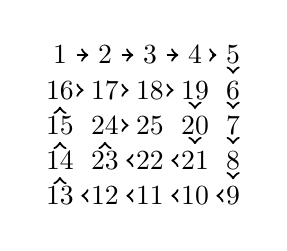
\begin{tikzpicture}
    % Creazione della matrice
    \matrix (m) [matrix of nodes, 
                  nodes={anchor=center},
                  column sep=-\pgflinewidth, row sep=-\pgflinewidth] 
    {
        1 & 2 & 3 & 4 & 5 \\
        16 & 17 & 18 & 19 & 6 \\
        15 & 24 & 25 & 20 & 7 \\
        14 & 23 & 22 & 21 & 8 \\
        13 & 12 & 11 & 10 & 9 \\
    };
    
    % Traccia il percorso
    % Colleghiamo i numeri 1 -> 2 -> 3 -> 4 -> 5 -> 6 -> 7 -> 8 -> 9
    \draw[->, thick] (m-1-1) -- (m-1-2);  % 1 -> 2
    \draw[->, thick] (m-1-2) -- (m-1-3);  % 2 -> 3
    \draw[->, thick] (m-1-3) -- (m-1-4);  % 3 -> 4
    \draw[->, thick] (m-1-4) -- (m-1-5);  % 4 -> 5
    
    \draw[->, thick] (m-2-5) -- (m-1-5);  % 5 -> 6
    \draw[->, thick] (m-3-5) -- (m-2-5);  % 6 -> 7
    \draw[->, thick] (m-4-5) -- (m-3-5);  % 7 -> 8
    \draw[->, thick] (m-5-5) -- (m-4-5);  % 8 -> 9
    
    % Poi il percorso ritorna indietro
    \draw[->, thick] (m-5-4) -- (m-5-5);  % 9 -> 10
    \draw[->, thick] (m-5-3) -- (m-5-4);  % 10 -> 11
    \draw[->, thick] (m-5-2) -- (m-5-3);  % 11 -> 12
    \draw[->, thick] (m-5-1) -- (m-5-2);  % 12 -> 13
    
    \draw[->, thick] (m-4-1) -- (m-5-1);  % 13 -> 14
    \draw[->, thick] (m-3-1) -- (m-4-1);  % 14 -> 15
    \draw[->, thick] (m-2-1) -- (m-3-1);  % 15 -> 16
    
    \draw[->, thick] (m-2-2) -- (m-2-1);
    \draw[->, thick] (m-2-3) -- (m-2-2);
    \draw[->, thick] (m-2-4) -- (m-2-3);
    
    \draw[->, thick] (m-3-4) -- (m-2-4);
    \draw[->, thick] (m-4-4) -- (m-3-4);
    
    \draw[->, thick] (m-4-3) -- (m-4-4);
    \draw[->, thick] (m-4-2) -- (m-4-3);
    
    \draw[->, thick] (m-3-2) -- (m-4-2);
    
    \draw[->, thick] (m-3-3) -- (m-3-2);
    
\end{tikzpicture}

\end{document}

